\documentclass[9pt,twocolumn,twoside]{pnas-new}
% Use the lineno option to display guide line numbers if required.
% chktex-file 1

\usepackage{graphicx}
\usepackage{colortbl}
\usepackage{xspace}
\usepackage{amsmath, amsfonts, amssymb, bbm}
% generated by dblp_models/g_report/src/report.ipynb; refresh with make report
% FourYear = summed final four years; Career = whole-career supplement
% QQ excludes zero totals; means/Gini use all totals; Percent values omit the percent sign
\newcommand{\DBLPNComplete}{510}
\newcommand{\DBLPFourYearStart}{17}
\newcommand{\DBLPFourYearEnd}{20}
\newcommand{\ModelSeed}{63}
\newcommand{\DBLPFourYearQQRtwo}{0.975}
\newcommand{\DBLPFourYearMeanTotal}{28.127}
\newcommand{\DBLPFourYearGini}{0.467}
\newcommand{\DBLPFourYearNPositive}{500}
\newcommand{\DBLPFourYearNZero}{10}
\newcommand{\DBLPFourYearZeroPercent}{2.0}
\newcommand{\DBLPCareerQQRtwo}{0.992}
\newcommand{\DBLPCareerMeanTotal}{152.995}
\newcommand{\DBLPCareerGini}{0.360}
\newcommand{\DBLPCareerNPositive}{510}
\newcommand{\DBLPCareerNZero}{0}
\newcommand{\DBLPCareerZeroPercent}{0.0}
\newcommand{\DBLPRankInitialFinal}{0.187}
\newcommand{\DBLPRankLagThreeFinal}{0.653}
\newcommand{\DBLPRankLagFiveFinal}{0.583}
\newcommand{\DBLPFinalYearZeroPercent}{14.1}
\newcommand{\ARWFourFourYearQQRtwo}{0.991}
\newcommand{\ARWFourFourYearMeanTotal}{26.897}
\newcommand{\ARWFourFourYearGini}{0.318}
\newcommand{\ARWFourFourYearNPositive}{10000}
\newcommand{\ARWFourFourYearNZero}{0}
\newcommand{\ARWFourFourYearZeroPercent}{0.0}
\newcommand{\ARWFourCareerQQRtwo}{1.000}
\newcommand{\ARWFourCareerMeanTotal}{147.036}
\newcommand{\ARWFourCareerGini}{0.183}
\newcommand{\ARWFourCareerNPositive}{10000}
\newcommand{\ARWFourCareerNZero}{0}
\newcommand{\ARWFourCareerZeroPercent}{0.0}
\newcommand{\ARWFourRankInitialFinal}{0.002}
\newcommand{\ARWFourRankLagThreeFinal}{0.203}
\newcommand{\ARWFourRankLagFiveFinal}{0.077}
\newcommand{\ARWFourFinalYearZeroPercent}{0.0}
\newcommand{\GRWFourYearQQRtwo}{0.984}
\newcommand{\GRWFourYearMeanTotal}{41454.511}
\newcommand{\GRWFourYearGini}{0.992}
\newcommand{\GRWFourYearNPositive}{9825}
\newcommand{\GRWFourYearNZero}{175}
\newcommand{\GRWFourYearZeroPercent}{1.8}
\newcommand{\GRWCareerQQRtwo}{0.957}
\newcommand{\GRWCareerMeanTotal}{56998.145}
\newcommand{\GRWCareerGini}{0.985}
\newcommand{\GRWCareerNPositive}{10000}
\newcommand{\GRWCareerNZero}{0}
\newcommand{\GRWCareerZeroPercent}{0.0}
\newcommand{\GRWRankInitialFinal}{0.140}
\newcommand{\GRWRankLagThreeFinal}{0.833}
\newcommand{\GRWRankLagFiveFinal}{0.742}
\newcommand{\GRWFinalYearZeroPercent}{10.9}
\newcommand{\AROneFourYearQQRtwo}{0.992}
\newcommand{\AROneFourYearMeanTotal}{27.948}
\newcommand{\AROneFourYearGini}{0.507}
\newcommand{\AROneFourYearNPositive}{9999}
\newcommand{\AROneFourYearNZero}{1}
\newcommand{\AROneFourYearZeroPercent}{0.0}
\newcommand{\AROneCareerQQRtwo}{0.999}
\newcommand{\AROneCareerMeanTotal}{155.612}
\newcommand{\AROneCareerGini}{0.288}
\newcommand{\AROneCareerNPositive}{10000}
\newcommand{\AROneCareerNZero}{0}
\newcommand{\AROneCareerZeroPercent}{0.0}
\newcommand{\AROneRankInitialFinal}{0.001}
\newcommand{\AROneRankLagThreeFinal}{0.246}
\newcommand{\AROneRankLagFiveFinal}{0.100}
\newcommand{\AROneFinalYearZeroPercent}{2.5}
\newcommand{\HurdleAROneFourYearQQRtwo}{0.932}
\newcommand{\HurdleAROneFourYearMeanTotal}{25.129}
\newcommand{\HurdleAROneFourYearGini}{0.448}
\newcommand{\HurdleAROneFourYearNPositive}{9855}
\newcommand{\HurdleAROneFourYearNZero}{145}
\newcommand{\HurdleAROneFourYearZeroPercent}{1.5}
\newcommand{\HurdleAROneCareerQQRtwo}{0.987}
\newcommand{\HurdleAROneCareerMeanTotal}{135.411}
\newcommand{\HurdleAROneCareerGini}{0.255}
\newcommand{\HurdleAROneCareerNPositive}{10000}
\newcommand{\HurdleAROneCareerNZero}{0}
\newcommand{\HurdleAROneCareerZeroPercent}{0.0}
\newcommand{\HurdleAROneRankInitialFinal}{-0.012}
\newcommand{\HurdleAROneRankLagThreeFinal}{0.309}
\newcommand{\HurdleAROneRankLagFiveFinal}{0.136}
\newcommand{\HurdleAROneFinalYearZeroPercent}{15.7}
\newcommand{\ARSixFourYearQQRtwo}{0.936}
\newcommand{\ARSixFourYearMeanTotal}{23.469}
\newcommand{\ARSixFourYearGini}{0.442}
\newcommand{\ARSixFourYearNPositive}{9648}
\newcommand{\ARSixFourYearNZero}{352}
\newcommand{\ARSixFourYearZeroPercent}{3.5}
\newcommand{\ARSixCareerQQRtwo}{0.934}
\newcommand{\ARSixCareerMeanTotal}{136.980}
\newcommand{\ARSixCareerGini}{0.330}
\newcommand{\ARSixCareerNPositive}{9999}
\newcommand{\ARSixCareerNZero}{1}
\newcommand{\ARSixCareerZeroPercent}{0.0}
\newcommand{\ARSixRankInitialFinal}{0.129}
\newcommand{\ARSixRankLagThreeFinal}{0.592}
\newcommand{\ARSixRankLagFiveFinal}{0.531}
\newcommand{\ARSixFinalYearZeroPercent}{16.5}
\newcommand{\SEHurdleFourYearQQRtwo}{0.973}
\newcommand{\SEHurdleFourYearMeanTotal}{28.800}
\newcommand{\SEHurdleFourYearGini}{0.460}
\newcommand{\SEHurdleFourYearNPositive}{9741}
\newcommand{\SEHurdleFourYearNZero}{259}
\newcommand{\SEHurdleFourYearZeroPercent}{2.6}
\newcommand{\SEHurdleCareerQQRtwo}{0.967}
\newcommand{\SEHurdleCareerMeanTotal}{151.488}
\newcommand{\SEHurdleCareerGini}{0.341}
\newcommand{\SEHurdleCareerNPositive}{9998}
\newcommand{\SEHurdleCareerNZero}{2}
\newcommand{\SEHurdleCareerZeroPercent}{0.0}
\newcommand{\SEHurdleRankInitialFinal}{0.159}
\newcommand{\SEHurdleRankLagThreeFinal}{0.611}
\newcommand{\SEHurdleRankLagFiveFinal}{0.553}
\newcommand{\SEHurdleFinalYearZeroPercent}{14.3}
\newcommand{\DBLPQQRtwo}{\DBLPFourYearQQRtwo}
\newcommand{\ARWFourQQRtwo}{\ARWFourFourYearQQRtwo}
\newcommand{\GRWQQRtwo}{\GRWFourYearQQRtwo}
\newcommand{\AROneQQRtwo}{\AROneFourYearQQRtwo}
\newcommand{\HurdleAROneQQRtwo}{\HurdleAROneFourYearQQRtwo}
\newcommand{\ARSixQQRtwo}{\ARSixFourYearQQRtwo}
\newcommand{\SEHurdleQQRtwo}{\SEHurdleFourYearQQRtwo}
\newcommand{\GRWLognormalRtwo}{\GRWFourYearQQRtwo}

\articletype{CLASSIFICATION}%%%% Article topic/classification

\templatetype{pnasresearcharticle} % Choose template
% {pnasresearcharticle} = Template for a two-column research article
% {pnasmathematics} %= Template for a one-column mathematics article
% {pnasinvited} %= Template for a PNAS invited submission


\begin{document}


\title{Unequal scientific productivity emerges from stochastic temporal processes}

% Use letters for affiliations, numbers to show equal authorship (if applicable) and to indicate the corresponding author
\author[a,1]{Samantha Magid}
\author[c]{Aanjaneya Kumar}
\author[d,c]{Daniel B. Larremore}
\author[d,c]{Aaron Clauset}
% Aanj
% Dan
% Aaron
\author[a,b,c,d,1,2]{Sam Zhang}

\affil[a]{Vermont Complex Systems Institute, University of Vermont, Burlington, VT 05405, USA.}
\affil[b]{Department of Mathematics and Statistics, University of Vermont, Burlington, VT 05405, USA.}
\affil[c]{Santa Fe Institute, Santa Fe, NM 87501, USA.}
\affil[d]{Department of Computer Science, University of Colorado Boulder, Boulder, CO 80309, USA}
% Please give the surname of the lead author for the running footer
\leadauthor{Magid}

% Please include corresponding author, author contribution and author declaration information
\authorcontributions{This is a placeholder for a description of the nature of SM and SZ contributions.}
\authordeclaration{The authors declare no competing interest.}
\equalauthors{\textsuperscript{1}Samantha Magid and Sam Zhang contributed equally to this work.}
\correspondingauthor{\textsuperscript{2}To whom correspondence should be addressed. E-mail: sam.zhang@uvm.edu.}



% At least three keywords are required at submission. Please provide three to five keywords, separated by the pipe symbol.
\keywords{Scientific productivity $|$ science of science $|$ stochastic processes $|$ temporal dynamics $|$ inequality}

\begin{abstract}
In 1957, Nobel Prize-winning physicist William Shockley suggested that the large individual differences in cumulative scientific productivity, which is approximately lognormally distributed, could be explained as the result of differences in fixed individual traits of scientific ability. However, the mathematical and methodological reasoning he provided fall short of supporting his suggestion. We identify and respond to these shortcomings. We iteratively develop several temporal models and empirical temporal dynamics against which to appraise them. We found that approximate cumulative lognormality was reproduced by every model we tested, regardless of how consistent the model was with other empirical constraints. Ultimately, we identify a self-exciting hurdle model which is consistent with both cumulative lognormality and our empirical temporal constraints. We show that stochastic temporal processes can generate unequal scientific productivity without invoking Shockley's assumption of fixed differences in individual scientific ability.
\end{abstract}

\dates{This manuscript was compiled on \today}
\doi{\url{www.pnas.org/cgi/doi/10.1073/pnas.XXXXXXXXXX}}


\maketitle
\thispagestyle{firststyle}
\ifthenelse{\boolean{shortarticle}}{\ifthenelse{\boolean{singlecolumn}}{\abscontentformatted}{\abscontent}}{}

\Firstpage
The study of scientific productivity heavily focuses on explaining the large differences publication counts between the most and least productive scientists. This inquiry began over a century ago with Lotka's Law of scientific productivity distribution~\cite{origins_of_productivity_frequency_law_lotka1926}. In the intervening century, the metascientific study of productivity has attracted scientists from a wide array of fields, all aiming to turn their focus inwards. Notably, in 1957, Nobel Prize-winning physicist William Shockley observed that some scientists are dramatically more productive than others, and posited an influential explanation for why that is~\cite{product_of_factors_explains_lognormality_shockley1957}. Specifically, the rate of publications and patents produced by researchers in Shockley's dataset followed an approximately lognormal distribution, a heavy-tailed distribution where a minority of scientists were significantly more productive than the rest. Shockley sought to explain this through stable differences in individual cognitive and managerial talent.
\subsection*{Shockley's idea}\label{subsec:intro_shockley}
He gave the following framework to explain his observation. For sufficiently large $n$, assuming finite variance and negligible contributions from extreme fluctuations to the total variance, the sum of independently varying factors can be approximately normally distributed. Because a sum of logarithms is the logarithm of a product, Shockley concluded that the lognormally distributed publication counts $P$ were the product of $k$ independently varying aspects of scientific ability $F$:
\begin{equation}
\log P = \sum_{i=1}^{k}\log F_i
\;\dot{\sim}\; \mathcal{N}(\mu,\sigma^2).
\label{eq:shockley_model}
\end{equation}
Shockley's contribution represented an influential proposal for an explanatory model of scientific productivity~\cite{shockley_in_modern_science_of_science_wang2021}. Despite its age and the author's subsequent vocal advocacy of eugenics, it has largely escaped scrutiny, and is frequently cited in modern scientific productivity research~\cite{called_shockley_elegant, impact_hot_streaks_and_disruptive_work_chen2025, franceschetSkewnessComputerScience2010, petersenPersistenceUncertaintyAcademic2012, sajindraTrackingHighImpactResearchers2026, petersenMethodsMeasuringCitations2010}. However, his model has several major shortcomings.
\Endparasplit
\subsection*{Atemporality}\label{subsec:intro_atemp}
This model is motivated by an ECDF regularity. However, it lacks a temporal component, despite the fact that the accumulation of publications inherently occurs over time. It therefore cannot explain any known temporal dynamics of scientific productivity. More fundamentally, explaining the distribution of accumulated output requires distinguishing the process of accumulation from the distribution it produces.
\subsection*{Non-identification}\label{subsec:intro_nonID}
Shockley infers a multiplicative structure from his observation that log productivity is approximately normally distributed. However, normality after taking logarithms does not establish that the underlying contributions combined multiplicatively: a lognormal distribution can also arise as a \emph{sum} of independent nonnegative random variables~\cite{thorinInfiniteDivisibilityLognormal1977}. Further, while cumulative lognormality can arise through multiplying components, that alone provides no basis for preferring his interpretation of those components as facets of procedural `ability' above anything else. 

\subsection*{Ideology of intrinsic human differences}\label{subsec:intro_eugenics}
Shockley, who would go on to gain notoriety for his advocacy of eugenicist beliefs, believed in the central importance of intelligence and other stable individual traits. He believed that scientific ability is generated by intelligence, and that intelligence is determined by immutable race and genetics, which intervention cannot meaningfully remediate~\cite{shockley_lectures_on_eugenics_and_research_taboos1967, shockley_public_hereditarian_and_eugenic_views1965, shockley_later_self_explanation_of_hereditarian_views1980}. His proposed explanation is in line \ldots

\section*{Empirical targets and model diagnostics}\label{sec:empirical_constraints}
To design temporal models, we first undertook exploratory data analysis of longitudinal publication records for 2,086 computer science researchers in the dblp computer science bibliography (`dblp dataset'). 

\begin{figure*}[t]
    \centering
    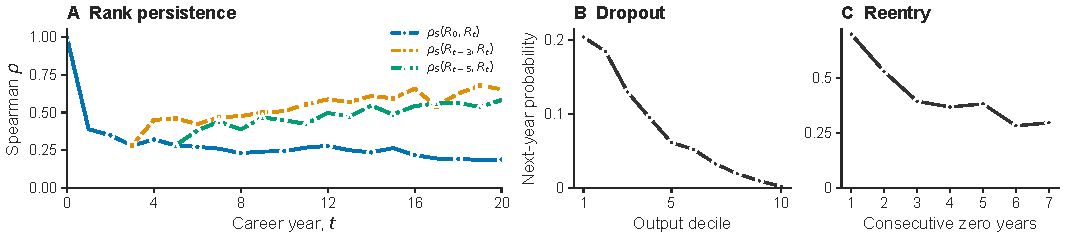
\includegraphics[width=\textwidth]{../../dblp_models/f_plot/output/pnas/pnas_dblp_temporal_wide.pdf}
    \caption{\textbf{Temporal patterns of publication in DBLP.}
    (A) Spearman correlations with year 0 ranks decline, while correlations at three- and five-year lags generally increase.
    (B) Among researchers who published in a given year, the probability of zero output the following year declines across current output deciles.
    (C) The probability of publishing the following year generally declines with the number of consecutive years of zero output.}\label{fig:dblp-rank-mixing}
\end{figure*}

We identified three temporal patterns in DBLP publication histories (Fig.~\ref{fig:dblp-rank-mixing}). Annual publication ranks became less aligned with career-year 0 ranks as careers progressed, while rank correlations at fixed three- and five-year lags generally strengthened. Among researchers who published in a given year, those with higher output were less likely to record zero output the following year. Among researchers with zero output, the probability of publishing the following year generally fell as the inactive spell lengthened. These patterns give temporal models of productivity three targets beyond the distribution of cumulative output that motivated Shockley's account.

We compared simulated and observed productivity using distributional and
temporal diagnostics. For publication totals in career years 17--20,
matching the length of Shockley's observation window, we report the
median, mean, standard deviation, and Gini coefficient, and assess
lognormality among positive totals using QQ $R^2$. We quantify agreement
in annual output using the Wasserstein-1 distance between simulated and
observed distributions at each career year. We average these distances
($\bar{W}_1$) over years 0--20 and also summarize them within the career
stages identified by Zhang et al.~\cite{random_walk_reproduces_productivity_trajectories_zhang2026}.
For each of the two rank-persistence curves (fixed year~0 and fixed
five-year lag), we report the Spearman correlation at endpoint year~20
and the OLS slope over endpoint years 17--20. We summarize agreement
with the dropout and reentry patterns illustrated in
Fig.~\ref{fig:dblp-rank-mixing}B--C using RMSE in percentage points.
Dropout errors are weighted by the observed number of active
researcher-years in each output bin. Reentry errors are weighted by
the observed number at risk at each duration, using durations with
at least 20 observed cases at risk.

\begin{table*}[t]
    \centering
    \caption{\textbf{Comparison of observed and simulated productivity.}
    The shaded row contains empirical dblp values. Slopes are changes in
    Spearman $\rho$ per career year, and RMSE is in percentage points (pp). Dashes indicate comparisons that use dblp as the reference.
    See \hyperref[sec:empirical_constraints]{Empirical targets and model diagnostics} for metric definitions.}\label{tab:model-comparison}
    \setlength{\tabcolsep}{4pt}
    \begin{tabular}{@{}lrrrrrrrrrrrr@{}}
        \toprule
        & \multicolumn{5}{c}{Final four years (17--20)}
        & & \multicolumn{4}{c}{Rank persistence} & \multicolumn{2}{c}{RMSE (pp)} \\
        \cmidrule(lr){2-6}\cmidrule(lr){8-11}
        \cmidrule(l){12-13}
        Model & QQ $R^2$ & Med. & Mean & SD & Gini
        & $\bar{W}_1$ & $\rho_S(R_0, R_{20})$ & Slope & $\rho_S(R_{15}, R_{20})$ & Slope & Dropout & Reentry \\
        \midrule
        \rowcolor{gray!12}
        \textit{dblp}
        & \DBLPFourYearQQRtwo & \DBLPFourYearMedianTotal
        & \DBLPFourYearMeanTotal & \DBLPFourYearSDTotal
        & \DBLPFourYearGini & \textemdash
        & \DBLPRankInitialFinal & \DBLPRankInitialFourYearSlope
        & \DBLPRankLagFiveFinal & \DBLPRankLagFiveFourYearSlope
        & \textemdash & \textemdash \\
        GRW
        & \GRWFourYearQQRtwo & \GRWFourYearMedianTotal
        & \GRWFourYearMeanTotal & \GRWFourYearSDTotal
        & \GRWFourYearGini & \GRWAnnualWassersteinMean
        & \GRWRankInitialFinal & \GRWRankInitialFourYearSlope
        & \GRWRankLagFiveFinal & \GRWRankLagFiveFourYearSlope
        & \GRWDropoutRMSEPoints & \GRWRestartHazardRMSEPoints \\
        AR(1)
        & \AROneFourYearQQRtwo & \AROneFourYearMedianTotal
        & \AROneFourYearMeanTotal & \AROneFourYearSDTotal
        & \AROneFourYearGini & \AROneAnnualWassersteinMean
        & \AROneRankInitialFinal & \AROneRankInitialFourYearSlope
        & \AROneRankLagFiveFinal & \AROneRankLagFiveFourYearSlope
        & \AROneDropoutRMSEPoints & \AROneRestartHazardRMSEPoints \\
        H-AR(1)
        & \HurdleAROneFourYearQQRtwo & \HurdleAROneFourYearMedianTotal
        & \HurdleAROneFourYearMeanTotal & \HurdleAROneFourYearSDTotal
        & \HurdleAROneFourYearGini & \HurdleAROneAnnualWassersteinMean
        & \HurdleAROneRankInitialFinal & \HurdleAROneRankInitialFourYearSlope
        & \HurdleAROneRankLagFiveFinal & \HurdleAROneRankLagFiveFourYearSlope
        & \HurdleAROneDropoutRMSEPoints & \HurdleAROneRestartHazardRMSEPoints \\
        HD-H
        & \SEHurdleFourYearQQRtwo & \SEHurdleFourYearMedianTotal
        & \SEHurdleFourYearMeanTotal & \SEHurdleFourYearSDTotal
        & \SEHurdleFourYearGini & \SEHurdleAnnualWassersteinMean
        & \SEHurdleRankInitialFinal & \SEHurdleRankInitialFourYearSlope
        & \SEHurdleRankLagFiveFinal & \SEHurdleRankLagFiveFourYearSlope
        & \SEHurdleDropoutRMSEPoints & \SEHurdleRestartHazardRMSEPoints \\
        \bottomrule
    \end{tabular}
\end{table*}

\section*{Temporal models}\label{sec:model}

We developed and tested several models of scientific productivity. Each model was developed in response to observed shortcomings in preceding models. Our models were designed by drawing from the literature of external fields with similar mathematical abstractions, including control theory, econometrics, and biostatistics, as well as from mathematical intuition about the nature of scientific productivity over time. Each model is fitted and evaluated against the dblp dataset using the above constraints and targets. For brevity, our reporting of results will refer to Table~\ref{tab:model-comparison}.

Models discussed in the main body of this report are generally fitted four times using the career change points (`stages') identified by Zhang et al.\ in their temporal analysis of the same dataset~\cite{random_walk_reproduces_productivity_trajectories_zhang2026}. 

\subsection*{Geometric Random Walk}\label{subsec:model_GRW}
We began with a geometric random walk (GRW) with IID lognormal multipliers. We fitted a single normal distribution to observed adjacent-year changes in log-offset productivity, pooled over the 20 career-year transitions, and exponentiated independent draws from that distribution.

\subsection*{Geometric Random Walk}\label{subsec:model_GRW}
We began with a geometric random walk (GRW) with IID lognormal multipliers. We fitted a single normal distribution to observed adjacent-year changes in log-offset productivity, pooled over the 20 career-year transitions, and exponentiated independent draws from that distribution.

The GRW generated approximately lognormal career totals, yet substantially misrepresented other empirical properties; four-year mean and standard deviation are catastrophically overestimated, while the four-year median is only overestimated by roughly double, indicative of an extremely overdispersed model; its simulated Gini was also roughly double the empirical value, and it overestimated fixed-distance rank correlation while underestimating fixed-point rank correlation.

Thus, reproducing approximate lognormality did not yield an adequate model of productivity. The GRW, then, provides a twofold counterexample to the uniqueness of Shockley's explanation: successive stochastic shocks can generate an approximately lognormal cumulative distribution without assigning researchers fixed differences in ability, and reproducing an approximately lognormal cumulative distribution identifies neither a specific nor a consistent model. This does not exclude contributions from individual traits or establish the GRW as a sufficient explanation; it demonstrates that distributional form alone cannot identify Shockley's proposed mechanism.

\subsection*{First-order autoregressive}\label{subsec_model_AR1}
The GRW's failure mode arises from the total persistence of shocks over time. In this view, it corresponds to the unit-persistence case ($\beta=1$) of the first-order autoregressive model $X_{t+1}=\alpha+\beta X_t+\epsilon_{t+1}$. To allow the effects of shocks to decay, and therefore reduce the overestimation of GRW, we fitted an $\operatorname{AR}(1)$ model in which $\alpha$ and $\beta$ were freely estimated within each career stage.

\begin{figure}[h]
    \centering
    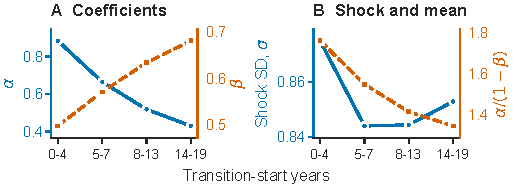
\includegraphics[width=\columnwidth]{../../dblp_models/f_plot/output/pnas/pnas_dblp_ar1_stage_parameters.pdf}
    \caption{Fitted $\operatorname{AR}(1)$ parameters by career stage.}\label{fig:ar1-stage-parameters}
\end{figure}

Across career stages, $\beta$ increased while $\alpha$ declined (Fig.~\ref{fig:ar1-stage-parameters}). The decline in $\alpha$ was large enough that the implied long-run mean, $\alpha/(1-\beta)$, fell on the log-offset scale. Shock variability was highest in the earliest stage and remained lower thereafter. Later-career shocks were thus modestly smaller and carried forward more strongly, a pattern consistent with the rise in fixed-lag rank correlations in Fig.~\ref{fig:dblp-rank-mixing}A.

The $\operatorname{AR}(1)$ retained approximate cumulative lognormality and brought the mean, median, and standard deviation of publication totals much closer to their empirical values, reducing $\bar{W}_1$ to less than two papers. Although its fixed-lag rank correlations increased over time, it substantially underpredicted both fixed-point and fixed-lag rank persistence. Its errors in dropout and reentry were also larger than those of the GRW, and it heavily underestimated the proportion of zero-publication streaks.

In processes involving count data where a model underestimates zero-count proportions, a hurdle model is a parsimonious choice~\cite{longitudinal_zero_and_positive_outcomes_farewell2017}. Taken together with Baccini et al.'s treatment of publishing/non-publishing as a  seperate process from publication intensity, we moved towards a hurdle autoregression model~\cite{bacciniCrossingHurdleDeterminants2014}.

\subsection*{Hurdle autoregressive}\label{subsec:model_hurdleAR}

To that end, we next fitted a hurdle autoregressive model H-AR(1) that separates whether a researcher publishes in a given year (`extensive margin') from how much they publish (`intensive margin'). This lets the probability of dropping to zero depend on current output and gives inactive researchers a separate probability of returning to publication. For researchers who continue publishing, output follows an autoregressive process. 

H-AR(1) saw marked improvement in empirical consistent over AR(1) in most metrics. It again produced approximate cumulative lognormality, although less so than any other model. It also yielded a significant reduction in dropout and reentry error. However, it still failed on long-run dynamics; by year 20 it retained scarce association with initial ranks, motivating us to include earlier history in prediction. 

\subsection*{History-dependent hurdle}\label{subsec:model_SE}

We retained the hurdle structure and allowed both margins to depend on earlier publication history, yielding a history-dependent hurdle model (HD-H). The rest of the model's design is motivated by parsimony. The extensive margin is a logistic regression due to its binary outcome; the conditional intensive margin is a linear regression with normal shocks. We incorporate earlier history as an exponentially weighted average up to $t-2$. This encodes the inductive bias that past output becomes less influential with time, with just one parameter needed to estimate the rate of decay.

HD-H's simulated results were highly empirically consistent. It reproduced approximate cumulative lognormality, returned a $\bar{W}_1$ of just over half a paper, and closely matched mean, median, standard deviation, and Gini. It also most closely reproduced the slopes of both fixed-distance and fixed-point rank persistence, and the Spearman $\rho$ of the former, but fell short of GRW in the latter. HD-H also reduced reentry error by approximately 85\%, but its dropout error worsened slightly relative to H-AR(1). 

Notably, HD-H's QQ $R^2$ error, the lowest among all the models, is slightly lower than the empirical value. In a test of the same statistic across 200 seeds, HD-H produced the closest $R^2$ 100\% of the time and remained below the empirical value 92.5\% of the time. Further, the second-most consistent model, H-AR(1), also 



We therefore examined the QQ residuals across quantiles to assess whether HD-H also reproduced the pattern of departures from lognormality observed in DBLP.

\begin{table}[H]
\centering
\begin{minipage}[t]{0.475\columnwidth}
    \vspace{0pt}
    \caption{Relative weight on earlier output in HD-H.
    For each margin, entries divide the coefficient on $H_t$ by
    that on last year's log-shifted output. A ratio of 1 indicates
    equal weight per unit.}\label{tab:seh-history-weight}
\end{minipage}%
\hspace{0.025\columnwidth}%
\begin{minipage}[t]{0.50\columnwidth}
    \vspace{0pt}
    \setlength{\tabcolsep}{3pt}
    \begin{tabular*}{\linewidth}{@{\extracolsep{\fill}}lrr@{}}
        \toprule
        Stage & Extensive & Intensive \\
        \midrule
        0--4   & \SEHurdleHistoryRatioExtensiveStageOne
               & \SEHurdleHistoryRatioIntensiveStageOne \\
        5--7   & \SEHurdleHistoryRatioExtensiveStageTwo
               & \SEHurdleHistoryRatioIntensiveStageTwo \\
        8--13  & \SEHurdleHistoryRatioExtensiveStageThree
               & \SEHurdleHistoryRatioIntensiveStageThree \\
        14--19 & \SEHurdleHistoryRatioExtensiveStageFour
               & \SEHurdleHistoryRatioIntensiveStageFour \\
        \bottomrule
    \end{tabular*}
\end{minipage}
\end{table}

We found that, when treated as a predictor in both margins, the history term was weighted in rough parity to the productivity of the previous year, except in the first stage. 





\section*{Discussion}


Our results show that approximate lognormality places only limited constraints on explanations of scientific productivity. Models with substantially different temporal structures generated approximately lognormal career totals while differing markedly in output levels, inequality, inactivity, and rank persistence. The GRW illustrates this distinction: a temporal multiplicative process reproduced the broad distributional form invoked by Shockley while failing other empirical checks. Lognormality therefore cannot, by itself, identify stable individual traits as the underlying mechanism. This finding does not establish that individual differences are irrelevant; it limits what can be inferred about them from cumulative publication distributions.

Our complementary analyses of the AARC panel, comprising 92,527 faculty across 113 fields, identify additional constraints on explanatory models. Publication activity was more temporally clustered than under shuffled histories, relative productivity ranks retained substantial memory, and the probability of returning to publication declined with the duration of inactivity. Evidence against a first-order Markov description further indicates that current annual output does not contain all available predictive information about subsequent productivity. Together, these findings suggest that productivity reflects persistent states or accumulated history that annual publication counts only partially reveal. Their prevalence and variation across fields can help distinguish general features of research production from effects associated with particular disciplinary practices.

The improved agreement of the self-exciting hurdle model is consistent with this interpretation. Incorporating earlier productivity into both publication activity and positive output brought simulated rank persistence, inactivity, and inequality closer to their empirical values. However, predictive dependence on publication history does not establish that publications themselves cause subsequent productivity. Earlier output may instead reflect unobserved project inventories, collaborations, resources, institutional conditions, or persistent individual differences. The history term summarizes these possibilities without distinguishing among them.

An explanatory model therefore requires mechanisms beyond the temporal regressions we considered here. These models describe how observed output depends statistically on earlier output, but they do not represent how research projects are initiated, developed, abandoned, and completed. A mechanistic model could instead allocate a finite effort budget among unfinished projects, with publications emerging upon completion. Project accumulation, heterogeneous completion times, interruptions, and collaboration could then generate temporal clustering, inactivity, and persistent productivity differences. Such mechanisms would permit tests of whether these regularities arise without fixed differences in researcher ability, and how individual differences interact with stochastic research processes.

Future work should evaluate these mechanisms jointly against CDFs and temporal diagnostics, including rank memory, inactivity-duration-dependent reentry, and publication clustering. Field-specific comparisons could test whether shared mechanisms with different timescales account for disciplinary variation. Stronger evaluation also requires common fitting cohorts, held-out researchers and career periods, uncertainty estimates, and sensitivity to initialization, observation windows, and the treatment of zero output. Publication inactivity must also be distinguished from research inactivity, since publication records cannot completely observe the underlying work.



% discussion and concluding paragraph go here

% bibliography uses references.bib
\Endparasplit
\subsection*{Supporting Information Appendix (SI)}

Authors should submit SI as a single separate SI Appendix PDF file, combining all text, figures, tables, movie legends, and SI references. SI will be published as provided by the authors; it will not be edited or composed. Additional details can be found in the \href{https://www.pnas.org/author-center/submitting-your-manuscript#supporting-information}{PNAS Author Center}. The PNAS Overleaf SI template can be found \href{https://www.overleaf.com/latex/templates/pnas-template-for-supplementary-information/wqfsfqwyjtsd}{here}. Refer to the SI Appendix in the manuscript at an appropriate point in the text. Number supporting figures and tables starting with S1, S2, etc.

Authors who place detailed materials and methods in an SI Appendix must provide sufficient detail in the main text methods to enable a reader to follow the logic of the procedures and results and also must reference the SI methods. If a paper is fundamentally a study of a new method or technique, then the methods must be described completely in the main text.

Supporting information (SI) for PNAS Brief Reports is limited to extended methods, essential supporting datasets, software, and video/audio files; supporting text, tables or figures are not permitted.

\subsubsection*{SI Datasets}

Supply .xlsx, .csv, .txt, .rtf, GZ or .pdf files. This file type will be published in raw format and will not be edited or composed.

\matmethods{Please describe your materials and methods here. This can be more than one paragraph, and may contain subsections and equations as required. If your research involved human or animal participants, please identify the institutional review board and/or licensing committee that approved the experiments. Please also include a brief description of your informed consent procedure if your experiments involved human participants.}


\showmatmethods{} % Display the Materials and Methods section

\dataavail{To allow others to replicate and build on work published in PNAS, authors must make materials, data, and associated protocols, including code and scripts, available to readers in a public repository upon publication. Restrictions on full or partial access to these materials and requests for legal, ethical, and logistical (e.g., size) exceptions must be noted at submission. If requested, these materials must be made available to editors and reviewers during submission for the purpose of evaluating the manuscript. A statement detailing sharing plans will be included in the published article as provided within the submission form. Research datasets, whether original or previously published, must be cited in the references as a condition for publication. Please refer to our full \href{https://www.pnas.org/author-center/editorial-and-journal-policies\#materials-and-data-availability}{policy}.}

\acknow{The authors thank William H.W. Thompson, Dr.\ Laurent Hébert-Dufresne, Dr.\ Calla Glavin Beauregard, and Alejandro Javier Ruiz Iglesias for their invaluable insights in support of this work.}

\showacknow{} % Display the acknowledgments section




\bibsplit[3]
%Use \bibsplit to split the references from the body of the text. Value "[3]" represents the number of reference in the left column (Note: Please avoid single column figures & tables on this page.)

% Bibliography
\bibliography{references}

\end{document}
